    
    
    
    

    

    \hypertarget{gestion-de-sous-process}{%
\section{Gestion de sous-process}\label{gestion-de-sous-process}}

    \hypertarget{compluxe9ment---niveau-truxe8s-avancuxe9}{%
\subsection{Complément - niveau (très)
avancé}\label{compluxe9ment---niveau-truxe8s-avancuxe9}}

    Dans ce second notebook, nous allons étudier un deuxième programme
Python, que j'appelle \texttt{game.py} (en fait c'est le présent
notebook).

    \hypertarget{fonctions-de-game.py}{%
\subsubsection{\texorpdfstring{Fonctions de
\texttt{game.py}}{Fonctions de game.py}}\label{fonctions-de-game.py}}

    Son travail va consister à faire plusieurs choses en même temps~; pour
rester le plus simple possible, on va se contenter des trois fonctions
suivantes~:

\begin{itemize}
\tightlist
\item
  \emph{scheduler} (chef d'orchestre)~: on veut lancer à des moments
  préprogrammés des instances (sous-process) de \texttt{players.py}~;
\item
  \emph{multiplexer} (agrégateur)~: on veut lire et imprimer au fur et à
  mesure les messages émis par les sous-processus~;
\item
  horloge~: on veut également afficher chaque seconde le temps écoulé
  depuis le début.
\end{itemize}

    En pratique, le programme \texttt{game.py} serait plutôt le serveur du
jeu qui reçoit les mouvements de tous les joueurs, et diffuse ensuite en
retour, en mode broadcast, un état du jeu à tous les participants.

    Mais dans notre version hyper simpliste, ça donne un comportement que
j'ai essayé d'illustrer comme ceci~:

    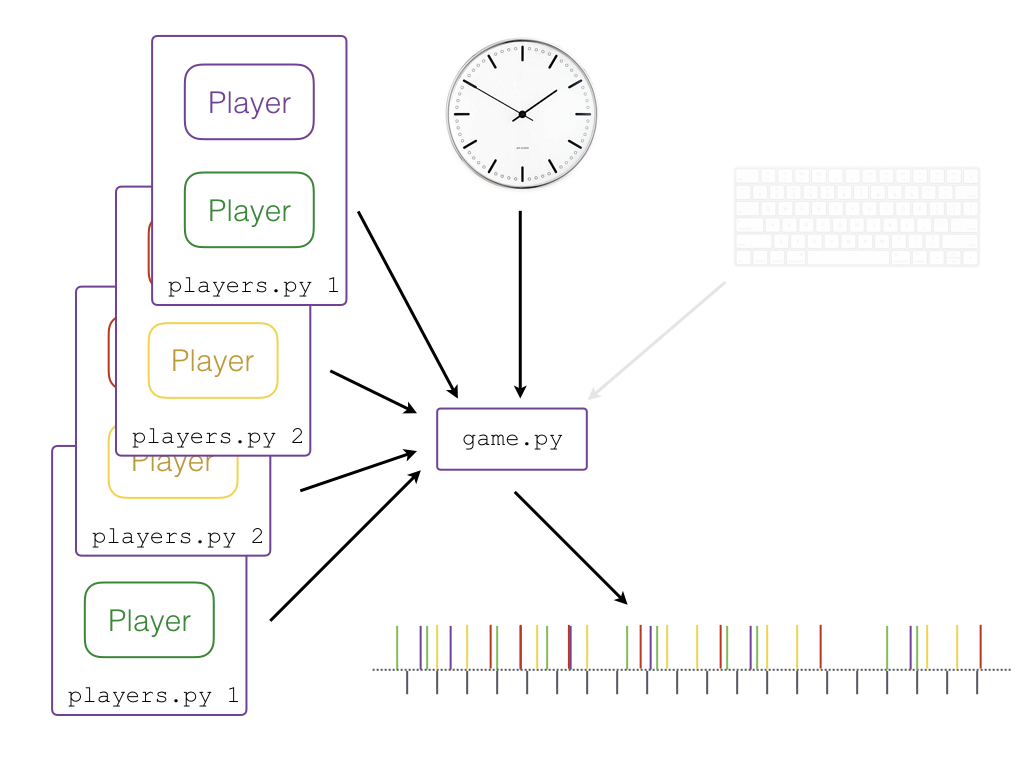
\includegraphics{media/game.png}

    \hypertarget{remarque-concernant-les-notebooks-et-le-clavier}{%
\subparagraph{Remarque concernant les notebooks et le
clavier}\label{remarque-concernant-les-notebooks-et-le-clavier}}

    Lorsqu'on exécute du code Python dans un notebook, les entrées clavier
sont en fait interceptées par le navigateur Web~; du coup on ne peut pas
facilement (du tout~?) faire tourner dans un notebook un programme
asynchrone qui réagirait aussi aux événements de type entrée clavier.

C'est pour cette raison que le clavier apparaît sur ma figure en
filigrane. Si vous allez jusqu'à exécuter ce notebook localement sur
votre machine (voir plus bas), vous pourrez utiliser le clavier pour
ajouter à la volée des éléments dans le scénario - en entrant des
numéros de 1 à 4 au moment voulu.

    \hypertarget{terminaison}{%
\subparagraph{Terminaison}\label{terminaison}}

    Pour rester simple et en l'absence de clavier, j'ai choisi de terminer
le programme lorsque le dernier sous-processus se termine.

    \hypertarget{le-programme-game.py}{%
\subsubsection{\texorpdfstring{Le programme
\texttt{game.py}}{Le programme game.py}}\label{le-programme-game.py}}

    C'est ce notebook qui va jouer pour nous le rôle du programme
\texttt{game.py}.

    \begin{Verbatim}[commandchars=\\\{\},frame=single,framerule=0.3mm,rulecolor=\color{cellframecolor}]
{\color{incolor}In [{\color{incolor}1}]:} \PY{k+kn}{import} \PY{n+nn}{asyncio}
        \PY{k+kn}{import} \PY{n+nn}{sys}
\end{Verbatim}


    \begin{Verbatim}[commandchars=\\\{\},frame=single,framerule=0.3mm,rulecolor=\color{cellframecolor}]
{\color{incolor}In [{\color{incolor}2}]:} \PY{c+c1}{\PYZsh{} cette constante est utile pour déclarer qu\PYZsq{}on a l\PYZsq{}intention}
        \PY{c+c1}{\PYZsh{} de lire les sorties (stout et stderr)}
        \PY{c+c1}{\PYZsh{} de nos sous\PYZhy{}process par l\PYZsq{}intermédiaire de pipes}
        \PY{k+kn}{from} \PY{n+nn}{subprocess} \PY{k}{import} \PY{n}{PIPE}
\end{Verbatim}


    Commençons par la classe \texttt{Scheduler}~; c'est celle qui va se
charger de lancer les sous-process selon un scénario. Pour ne pas se
compliquer la vie on choisit de représenter un scénario (un script)
comme une liste de tuples de la forme~:

\begin{Shaded}
\begin{Highlighting}[frame=lines,framerule=0.6mm,rulecolor=\color{asisframecolor}]
\NormalTok{script }\OperatorTok{=}\NormalTok{ [ (secondes, predef), ...]}
\end{Highlighting}
\end{Shaded}

qui signifie de lancer, un délai de \texttt{secondes} secondes après le
début du programme, le programme \texttt{players.py} dans la
configuration \texttt{predef} - de 1 à 4 donc.

    \begin{Verbatim}[commandchars=\\\{\},frame=single,framerule=0.3mm,rulecolor=\color{cellframecolor}]
{\color{incolor}In [{\color{incolor}3}]:} \PY{k}{class} \PY{n+nc}{Scheduler}\PY{p}{:}
        
            \PY{k}{def} \PY{n+nf}{\PYZus{}\PYZus{}init\PYZus{}\PYZus{}}\PY{p}{(}\PY{n+nb+bp}{self}\PY{p}{,} \PY{n}{script}\PY{p}{)}\PY{p}{:}
        
                \PY{c+c1}{\PYZsh{} on trie le script par ordre chronologique}
                \PY{n+nb+bp}{self}\PY{o}{.}\PY{n}{script} \PY{o}{=} \PY{n+nb}{list}\PY{p}{(}\PY{n}{script}\PY{p}{)}
                \PY{n+nb+bp}{self}\PY{o}{.}\PY{n}{script}\PY{o}{.}\PY{n}{sort}\PY{p}{(}\PY{n}{key} \PY{o}{=} \PY{k}{lambda} \PY{n}{time\PYZus{}predef} \PY{p}{:} \PY{n}{time\PYZus{}predef}\PY{p}{[}\PY{l+m+mi}{0}\PY{p}{]}\PY{p}{)}
        
                \PY{c+c1}{\PYZsh{} juste pour donner un numéro à chaque processus}
                \PY{n+nb+bp}{self}\PY{o}{.}\PY{n}{counter} \PY{o}{=} \PY{l+m+mi}{1}
                \PY{c+c1}{\PYZsh{} combien de processus sont actifs}
                \PY{n+nb+bp}{self}\PY{o}{.}\PY{n}{running} \PY{o}{=} \PY{l+m+mi}{0}
        
            \PY{k}{async} \PY{k}{def} \PY{n+nf}{run}\PY{p}{(}\PY{n+nb+bp}{self}\PY{p}{)}\PY{p}{:}
                \PY{l+s+sd}{\PYZdq{}\PYZdq{}\PYZdq{}}
        \PY{l+s+sd}{        fait tout le travail, c\PYZsq{}est\PYZhy{}à\PYZhy{}dire :}
        \PY{l+s+sd}{        * lance tous les sous\PYZhy{}processus à l\PYZsq{}heure indiquée}
        \PY{l+s+sd}{        * et aussi en préambule, pour le mode avec clavier,}
        \PY{l+s+sd}{          arme une callback sur l\PYZsq{}entrée standard}
        \PY{l+s+sd}{        \PYZdq{}\PYZdq{}\PYZdq{}}
                \PY{c+c1}{\PYZsh{} pour le mode avec clavier (pas fonctionnel dans le notebook)}
                \PY{c+c1}{\PYZsh{} on arme une callback sur stdin}
                \PY{n}{asyncio}\PY{o}{.}\PY{n}{get\PYZus{}event\PYZus{}loop}\PY{p}{(}\PY{p}{)}\PY{o}{.}\PY{n}{add\PYZus{}reader}\PY{p}{(}
                    \PY{c+c1}{\PYZsh{} il nous faut un file descriptor, pas un objet Python}
                    \PY{n}{sys}\PY{o}{.}\PY{n}{stdin}\PY{o}{.}\PY{n}{fileno}\PY{p}{(}\PY{p}{)}\PY{p}{,}
                    \PY{c+c1}{\PYZsh{} la callback}
                    \PY{n}{Scheduler}\PY{o}{.}\PY{n}{read\PYZus{}keyboard\PYZus{}line}\PY{p}{,}
                    \PY{c+c1}{\PYZsh{} les arguments de la callback}
                    \PY{c+c1}{\PYZsh{} cette fois c\PYZsq{}est un objet Python}
                    \PY{n+nb+bp}{self}\PY{p}{,} \PY{n}{sys}\PY{o}{.}\PY{n}{stdin}
                \PY{p}{)}
                \PY{c+c1}{\PYZsh{} le scénario prédéfini}
                \PY{n}{epoch} \PY{o}{=} \PY{l+m+mi}{0}
                \PY{k}{for} \PY{n}{tick}\PY{p}{,} \PY{n}{predef} \PY{o+ow}{in} \PY{n+nb+bp}{self}\PY{o}{.}\PY{n}{script}\PY{p}{:}
                    \PY{c+c1}{\PYZsh{} attendre le bon moment}
                    \PY{k}{await} \PY{n}{asyncio}\PY{o}{.}\PY{n}{sleep}\PY{p}{(}\PY{n}{tick} \PY{o}{\PYZhy{}} \PY{n}{epoch}\PY{p}{)}
                    \PY{c+c1}{\PYZsh{} pour le prochain}
                    \PY{n}{epoch} \PY{o}{=} \PY{n}{tick}
                    \PY{n}{asyncio}\PY{o}{.}\PY{n}{ensure\PYZus{}future}\PY{p}{(}\PY{n+nb+bp}{self}\PY{o}{.}\PY{n}{fork\PYZus{}players}\PY{p}{(}\PY{n}{predef}\PY{p}{)}\PY{p}{)}
        
            \PY{k}{async} \PY{k}{def} \PY{n+nf}{fork\PYZus{}players}\PY{p}{(}\PY{n+nb+bp}{self}\PY{p}{,} \PY{n}{predef}\PY{p}{)}\PY{p}{:}
                \PY{l+s+sd}{\PYZdq{}\PYZdq{}\PYZdq{}}
        \PY{l+s+sd}{        lance maintenant une instance de players avec cette config}
        
        \PY{l+s+sd}{        puis}
        \PY{l+s+sd}{        écoute à la fois sdtout et stderr, et les imprime}
        \PY{l+s+sd}{        (bon c\PYZsq{}est vrai que players n\PYZsq{}écrit rien sur stderr)}
        \PY{l+s+sd}{        attend la fin du sous\PYZhy{}processus (avec wait())}
        \PY{l+s+sd}{        et retourne son code de retour (exitcode) du sous\PYZhy{}processus}
        
        \PY{l+s+sd}{        par commodité on décide d\PYZsq{}arrêter la boucle principale}
        \PY{l+s+sd}{        lorsqu\PYZsq{}il n\PYZsq{}y a plus aucun process actif}
        \PY{l+s+sd}{        \PYZdq{}\PYZdq{}\PYZdq{}}
        
                \PY{c+c1}{\PYZsh{} la commande à lancer pour forker une instance de players.py}
                \PY{n}{command} \PY{o}{=} \PY{n}{f}\PY{l+s+s2}{\PYZdq{}}\PY{l+s+s2}{python3 \PYZhy{}u data/players.py }\PY{l+s+si}{\PYZob{}predef\PYZcb{}}\PY{l+s+s2}{\PYZdq{}}\PY{o}{.}\PY{n}{split}\PY{p}{(}\PY{p}{)}
                \PY{c+c1}{\PYZsh{} pour afficher un nom un peu plus parlant}
                \PY{n}{worker} \PY{o}{=} \PY{n}{f}\PY{l+s+s2}{\PYZdq{}}\PY{l+s+s2}{ps\PYZsh{}}\PY{l+s+si}{\PYZob{}self.counter\PYZcb{}}\PY{l+s+s2}{ (predef }\PY{l+s+si}{\PYZob{}predef\PYZcb{}}\PY{l+s+s2}{)}\PY{l+s+s2}{\PYZdq{}}
                \PY{c+c1}{\PYZsh{} housekeeping}
                \PY{n+nb+bp}{self}\PY{o}{.}\PY{n}{counter} \PY{o}{+}\PY{o}{=} \PY{l+m+mi}{1}
                \PY{n+nb+bp}{self}\PY{o}{.}\PY{n}{running} \PY{o}{+}\PY{o}{=} \PY{l+m+mi}{1}
                \PY{c+c1}{\PYZsh{} c\PYZsq{}est là que ça se passe : on forke}
                \PY{n+nb}{print}\PY{p}{(}\PY{l+m+mi}{8} \PY{o}{*} \PY{l+s+s1}{\PYZsq{}}\PY{l+s+s1}{\PYZgt{}}\PY{l+s+s1}{\PYZsq{}}\PY{p}{,} \PY{n}{f}\PY{l+s+s2}{\PYZdq{}}\PY{l+s+s2}{worker }\PY{l+s+si}{\PYZob{}worker\PYZcb{}}\PY{l+s+s2}{\PYZdq{}}\PY{p}{)}
                \PY{n}{process} \PY{o}{=} \PY{k}{await} \PY{n}{asyncio}\PY{o}{.}\PY{n}{create\PYZus{}subprocess\PYZus{}exec}\PY{p}{(}
                    \PY{o}{*}\PY{n}{command}\PY{p}{,}
                    \PY{n}{stdout}\PY{o}{=}\PY{n}{PIPE}\PY{p}{,} \PY{n}{stderr}\PY{o}{=}\PY{n}{PIPE}\PY{p}{,}
                \PY{p}{)}
                \PY{c+c1}{\PYZsh{} et on lit et écrit les canaux du sous\PYZhy{}process}
                \PY{n}{stdout}\PY{p}{,} \PY{n}{stderr} \PY{o}{=} \PY{k}{await} \PY{n}{asyncio}\PY{o}{.}\PY{n}{gather}\PY{p}{(}
                    \PY{n+nb+bp}{self}\PY{o}{.}\PY{n}{read\PYZus{}and\PYZus{}display}\PY{p}{(}\PY{n}{process}\PY{o}{.}\PY{n}{stdout}\PY{p}{,} \PY{n}{worker}\PY{p}{)}\PY{p}{,}
                    \PY{n+nb+bp}{self}\PY{o}{.}\PY{n}{read\PYZus{}and\PYZus{}display}\PY{p}{(}\PY{n}{process}\PY{o}{.}\PY{n}{stderr}\PY{p}{,} \PY{n}{worker}\PY{p}{)}\PY{p}{)}
                \PY{c+c1}{\PYZsh{} qu\PYZsq{}il ne faut pas oublier d\PYZsq{}attendre pour que l\PYZsq{}OS sache}
                \PY{c+c1}{\PYZsh{} qu\PYZsq{}il peut nettoyer}
                \PY{n}{retcod} \PY{o}{=} \PY{k}{await} \PY{n}{process}\PY{o}{.}\PY{n}{wait}\PY{p}{(}\PY{p}{)}
                \PY{c+c1}{\PYZsh{} le process est terminé}
                \PY{n+nb+bp}{self}\PY{o}{.}\PY{n}{running} \PY{o}{\PYZhy{}}\PY{o}{=} \PY{l+m+mi}{1}
                \PY{n+nb}{print}\PY{p}{(}\PY{l+m+mi}{8} \PY{o}{*} \PY{l+s+s1}{\PYZsq{}}\PY{l+s+s1}{\PYZlt{}}\PY{l+s+s1}{\PYZsq{}}\PY{p}{,} \PY{n}{f}\PY{l+s+s2}{\PYZdq{}}\PY{l+s+s2}{worker }\PY{l+s+si}{\PYZob{}worker\PYZcb{}}\PY{l+s+s2}{ \PYZhy{} exit code }\PY{l+s+si}{\PYZob{}retcod\PYZcb{}}\PY{l+s+s2}{\PYZdq{}}
                      \PY{n}{f}\PY{l+s+s2}{\PYZdq{}}\PY{l+s+s2}{ \PYZhy{} }\PY{l+s+si}{\PYZob{}self.running\PYZcb{}}\PY{l+s+s2}{ still running}\PY{l+s+s2}{\PYZdq{}}\PY{p}{)}
                \PY{c+c1}{\PYZsh{} si c\PYZsq{}était le dernier on sort de la boucle principale}
                \PY{k}{if} \PY{n+nb+bp}{self}\PY{o}{.}\PY{n}{running} \PY{o}{==} \PY{l+m+mi}{0}\PY{p}{:}
                    \PY{n+nb}{print}\PY{p}{(}\PY{l+s+s2}{\PYZdq{}}\PY{l+s+s2}{no process left \PYZhy{} bye}\PY{l+s+s2}{\PYZdq{}}\PY{p}{)}
                    \PY{n}{asyncio}\PY{o}{.}\PY{n}{get\PYZus{}event\PYZus{}loop}\PY{p}{(}\PY{p}{)}\PY{o}{.}\PY{n}{stop}\PY{p}{(}\PY{p}{)}
                \PY{c+c1}{\PYZsh{} sinon on retourne le code de retour}
                \PY{k}{return} \PY{n}{retcod}
        
            \PY{k}{async} \PY{k}{def} \PY{n+nf}{read\PYZus{}and\PYZus{}display}\PY{p}{(}\PY{n+nb+bp}{self}\PY{p}{,} \PY{n}{stream}\PY{p}{,} \PY{n}{worker}\PY{p}{)}\PY{p}{:}
                \PY{l+s+sd}{\PYZdq{}\PYZdq{}\PYZdq{}}
        \PY{l+s+sd}{        une coroutine pour afficher les sorties d\PYZsq{}un canal}
        \PY{l+s+sd}{        stdout ou stderr d\PYZsq{}un sous\PYZhy{}process}
        \PY{l+s+sd}{        retourne lorsque le process est terminé}
        \PY{l+s+sd}{        \PYZdq{}\PYZdq{}\PYZdq{}}
                \PY{k}{while} \PY{k+kc}{True}\PY{p}{:}
                    \PY{n+nb}{bytes} \PY{o}{=} \PY{k}{await} \PY{n}{stream}\PY{o}{.}\PY{n}{readline}\PY{p}{(}\PY{p}{)}
                    \PY{c+c1}{\PYZsh{} l\PYZsq{}OS nous signale qu\PYZsq{}on en a terminé}
                    \PY{c+c1}{\PYZsh{} avec ce process en renvoyant ici un objet bytes vide}
                    \PY{k}{if} \PY{o+ow}{not} \PY{n+nb}{bytes}\PY{p}{:}
                        \PY{k}{break}
                    \PY{c+c1}{\PYZsh{} ici on se contente d\PYZsq{}imprimer, du coup}
                    \PY{c+c1}{\PYZsh{} il faut convertir en str (bien qu\PYZsq{}ici}
                    \PY{c+c1}{\PYZsh{} players n\PYZsq{}écrit que de l\PYZsq{}ASCII)}
                    \PY{n}{line} \PY{o}{=} \PY{n+nb}{bytes}\PY{o}{.}\PY{n}{decode}\PY{p}{(}\PY{p}{)}\PY{o}{.}\PY{n}{strip}\PY{p}{(}\PY{p}{)}
                    \PY{n+nb}{print}\PY{p}{(}\PY{l+m+mi}{8} \PY{o}{*} \PY{l+s+s1}{\PYZsq{}}\PY{l+s+s1}{ }\PY{l+s+s1}{\PYZsq{}}\PY{p}{,} \PY{n}{f}\PY{l+s+s2}{\PYZdq{}}\PY{l+s+s2}{got `}\PY{l+s+si}{\PYZob{}line\PYZcb{}}\PY{l+s+s2}{` from }\PY{l+s+si}{\PYZob{}worker\PYZcb{}}\PY{l+s+s2}{\PYZdq{}}\PY{p}{)}
        
            \PY{c+c1}{\PYZsh{} ceci est seulement fonctionnel si vous exécutez}
            \PY{c+c1}{\PYZsh{} le programme localement sur votre ordinateur}
            \PY{c+c1}{\PYZsh{} car depuis un notebook le clavier est intercepté}
            \PY{c+c1}{\PYZsh{} par le serveur web}
            \PY{k}{def} \PY{n+nf}{read\PYZus{}keyboard\PYZus{}line}\PY{p}{(}\PY{n+nb+bp}{self}\PY{p}{,} \PY{n}{stdin}\PY{p}{)}\PY{p}{:}
                \PY{l+s+sd}{\PYZdq{}\PYZdq{}\PYZdq{}}
        \PY{l+s+sd}{        ceci est une callback; eh oui :)}
        \PY{l+s+sd}{        c\PYZsq{}est pourquoi d\PYZsq{}ailleurs ce n\PYZsq{}est pas une coroutine}
        \PY{l+s+sd}{        cependant on est sûr qu\PYZsq{}elle n\PYZsq{}est appelée}
        \PY{l+s+sd}{        que lorsqu\PYZsq{}il y a réellement quelque chose à lire}
        \PY{l+s+sd}{        \PYZdq{}\PYZdq{}\PYZdq{}}
                \PY{n}{line} \PY{o}{=} \PY{n}{stdin}\PY{o}{.}\PY{n}{readline}\PY{p}{(}\PY{p}{)}\PY{o}{.}\PY{n}{strip}\PY{p}{(}\PY{p}{)}
                \PY{c+c1}{\PYZsh{} ici je triche complètement}
                \PY{c+c1}{\PYZsh{} lorsqu\PYZsq{}on est dans un notebook, pour bien faire}
                \PY{c+c1}{\PYZsh{} on ne devrait pas regarder stdin du tout}
                \PY{c+c1}{\PYZsh{} mais pour garder le code le plus simple possible}
                \PY{c+c1}{\PYZsh{} je choisis d\PYZsq{}ignorer les lignes vides ici}
                \PY{c+c1}{\PYZsh{} comme ça mon code marche dans les deux cas}
                \PY{k}{if} \PY{o+ow}{not} \PY{n}{line}\PY{p}{:}
                    \PY{k}{return}
                \PY{c+c1}{\PYZsh{} on traduit la ligne tapée au clavier}
                \PY{c+c1}{\PYZsh{} en un entier entre 1 et 4}
                \PY{k}{try}\PY{p}{:}
                    \PY{n}{predef} \PY{o}{=} \PY{n+nb}{int}\PY{p}{(}\PY{n}{line}\PY{p}{)}
                    \PY{k}{if} \PY{o+ow}{not} \PY{p}{(}\PY{l+m+mi}{1} \PY{o}{\PYZlt{}}\PY{o}{=} \PY{n}{predef} \PY{o}{\PYZlt{}}\PY{o}{=} \PY{l+m+mi}{4}\PY{p}{)}\PY{p}{:}
                        \PY{k}{raise} \PY{n+ne}{ValueError}\PY{p}{(}\PY{l+s+s1}{\PYZsq{}}\PY{l+s+s1}{entre 1 et 4}\PY{l+s+s1}{\PYZsq{}}\PY{p}{)}
                \PY{k}{except} \PY{n+ne}{Exception} \PY{k}{as} \PY{n}{e}\PY{p}{:}
                    \PY{n+nb}{print}\PY{p}{(}\PY{n}{f}\PY{l+s+s2}{\PYZdq{}}\PY{l+s+si}{\PYZob{}line\PYZcb{}}\PY{l+s+s2}{ doit être entre 1 et 4 }\PY{l+s+s2}{\PYZob{}}\PY{l+s+s2}{type(e)\PYZcb{} \PYZhy{} }\PY{l+s+si}{\PYZob{}e\PYZcb{}}\PY{l+s+s2}{\PYZdq{}}\PY{p}{)}
                    \PY{k}{return}
                \PY{n}{asyncio}\PY{o}{.}\PY{n}{ensure\PYZus{}future}\PY{p}{(}\PY{n+nb+bp}{self}\PY{o}{.}\PY{n}{fork\PYZus{}players}\PY{p}{(}\PY{n}{predef}\PY{p}{)}\PY{p}{)}
\end{Verbatim}


    À ce stade on a déjà le cœur de la logique du \emph{scheduler}, et aussi
du multiplexer. Il ne nous manque plus que l'horloge~:

    \begin{Verbatim}[commandchars=\\\{\},frame=single,framerule=0.3mm,rulecolor=\color{cellframecolor}]
{\color{incolor}In [{\color{incolor}4}]:} \PY{k}{class} \PY{n+nc}{Clock}\PY{p}{:}
        
            \PY{k}{def} \PY{n+nf}{\PYZus{}\PYZus{}init\PYZus{}\PYZus{}}\PY{p}{(}\PY{n+nb+bp}{self}\PY{p}{)}\PY{p}{:}
                \PY{n+nb+bp}{self}\PY{o}{.}\PY{n}{clock\PYZus{}seconds} \PY{o}{=} \PY{l+m+mi}{0}
        
            \PY{k}{async} \PY{k}{def} \PY{n+nf}{run}\PY{p}{(}\PY{n+nb+bp}{self}\PY{p}{)}\PY{p}{:}
                \PY{k}{while} \PY{k+kc}{True}\PY{p}{:}
                    \PY{n+nb}{print}\PY{p}{(}\PY{n}{f}\PY{l+s+s2}{\PYZdq{}}\PY{l+s+s2}{clock = }\PY{l+s+si}{\PYZob{}self.clock\PYZus{}seconds:04d\PYZcb{}}\PY{l+s+s2}{s}\PY{l+s+s2}{\PYZdq{}}\PY{p}{)}
                    \PY{k}{await} \PY{n}{asyncio}\PY{o}{.}\PY{n}{sleep}\PY{p}{(}\PY{l+m+mi}{1}\PY{p}{)}
                    \PY{n+nb+bp}{self}\PY{o}{.}\PY{n}{clock\PYZus{}seconds} \PY{o}{+}\PY{o}{=} \PY{l+m+mi}{1}
\end{Verbatim}


    Et enfin pour mettre tous ces morceaux en route il nous faut une boucle
d'événements~:

    \begin{Verbatim}[commandchars=\\\{\},frame=single,framerule=0.3mm,rulecolor=\color{cellframecolor}]
{\color{incolor}In [{\color{incolor}5}]:} \PY{k}{class} \PY{n+nc}{Game}\PY{p}{:}
        
            \PY{k}{def} \PY{n+nf}{\PYZus{}\PYZus{}init\PYZus{}\PYZus{}}\PY{p}{(}\PY{n+nb+bp}{self}\PY{p}{,} \PY{n}{script}\PY{p}{)}\PY{p}{:}
                \PY{n+nb+bp}{self}\PY{o}{.}\PY{n}{script} \PY{o}{=} \PY{n}{script}
        
            \PY{k}{def} \PY{n+nf}{mainloop}\PY{p}{(}\PY{n+nb+bp}{self}\PY{p}{)}\PY{p}{:}
                \PY{n}{loop} \PY{o}{=} \PY{n}{asyncio}\PY{o}{.}\PY{n}{get\PYZus{}event\PYZus{}loop}\PY{p}{(}\PY{p}{)}
        
                \PY{n}{clock} \PY{o}{=} \PY{n}{Clock}\PY{p}{(}\PY{p}{)}
                \PY{n}{asyncio}\PY{o}{.}\PY{n}{ensure\PYZus{}future}\PY{p}{(}\PY{n}{clock}\PY{o}{.}\PY{n}{run}\PY{p}{(}\PY{p}{)}\PY{p}{)}
        
                \PY{n}{scheduler} \PY{o}{=} \PY{n}{Scheduler}\PY{p}{(}\PY{n+nb+bp}{self}\PY{o}{.}\PY{n}{script}\PY{p}{)}
                \PY{n}{asyncio}\PY{o}{.}\PY{n}{ensure\PYZus{}future}\PY{p}{(}\PY{n}{scheduler}\PY{o}{.}\PY{n}{run}\PY{p}{(}\PY{p}{)}\PY{p}{)}
                \PY{n}{loop}\PY{o}{.}\PY{n}{run\PYZus{}forever}\PY{p}{(}\PY{p}{)}
\end{Verbatim}


    Et maintenant je peux lancer une session simple~; pour ne pas être noyé
par les sorties on va se contenter de lancer~:

\begin{itemize}
\tightlist
\item
  0.5 seconde après le début une instance de \texttt{players.py\ 1}
\item
  1 seconde après le début une instance de \texttt{players.py\ 2}
\end{itemize}

    \begin{Verbatim}[commandchars=\\\{\},frame=single,framerule=0.3mm,rulecolor=\color{cellframecolor}]
{\color{incolor}In [{\color{incolor}6}]:} \PY{n}{game} \PY{o}{=} \PY{n}{Game}\PY{p}{(} \PY{p}{[}\PY{p}{(}\PY{l+m+mf}{0.5}\PY{p}{,} \PY{l+m+mi}{1}\PY{p}{)}\PY{p}{,} \PY{p}{(}\PY{l+m+mf}{1.}\PY{p}{,} \PY{l+m+mi}{2}\PY{p}{)}\PY{p}{]}\PY{p}{)}
        \PY{n}{game}\PY{o}{.}\PY{n}{mainloop}\PY{p}{(}\PY{p}{)}
\end{Verbatim}


    \begin{Verbatim}[commandchars=\\\{\},frame=single,framerule=0.3mm,rulecolor=\color{cellframecolor}]
clock = 0000s
>>>>>>>> worker ps\#1 (predef 1)
         got `S john` from ps\#1 (predef 1)
         got `W mary` from ps\#1 (predef 1)
         got `N mary` from ps\#1 (predef 1)
clock = 0001s
>>>>>>>> worker ps\#2 (predef 2)
         got `S mary` from ps\#1 (predef 1)
         got `W bill` from ps\#2 (predef 2)
         got `S jane` from ps\#2 (predef 2)
         got `E jane` from ps\#2 (predef 2)
         got `N mary` from ps\#1 (predef 1)
         got `S john` from ps\#1 (predef 1)
         got `S bill` from ps\#2 (predef 2)
         got `W jane` from ps\#2 (predef 2)
         got `S mary` from ps\#1 (predef 1)
         got `N john` from ps\#1 (predef 1)
         got `S jane` from ps\#2 (predef 2)
         got `W mary` from ps\#1 (predef 1)
         got `N bill` from ps\#2 (predef 2)
clock = 0002s
         got `W jane` from ps\#2 (predef 2)
         got `E mary` from ps\#1 (predef 1)
         got `W john` from ps\#1 (predef 1)
         got `W bill` from ps\#2 (predef 2)
         got `W mary` from ps\#1 (predef 1)
<<<<<<<< worker ps\#1 (predef 1) - exit code 0 - 1 still running
         got `S bill` from ps\#2 (predef 2)
         got `S bill` from ps\#2 (predef 2)
clock = 0003s
<<<<<<<< worker ps\#2 (predef 2) - exit code 0 - 0 still running
no process left - bye
\end{Verbatim}

    \hypertarget{conclusion}{%
\subsubsection{Conclusion}\label{conclusion}}

    Notre but avec cet exemple est de vous montrer, après les exemples des
vidéos qui reposent en grande majorité sur \texttt{asyncio.sleep}, que
la boucle d'événements de \texttt{asyncio} permet d'avoir accès, de
manière simple et efficace, à des événements de niveau OS. Dans un
complément précédent nous avions aperçu la gestion de requêtes HTTP~;
ici nous avons illustré la gestion de sous-process.

Actuellement on peut trouver des bibliothèques au dessus de
\texttt{asyncio} pour manipuler de cette façon quasiment tous les
protocoles réseau, et autres accès à des bases de données.

    \hypertarget{exuxe9cution-en-local}{%
\subsubsection{Exécution en local}\label{exuxe9cution-en-local}}

    Si vous voulez exécuter ce code localement sur votre machine~:

Tout d'abord sachez que je n'ai pas du tout essayé ceci sur un OS
Windows - et d'ailleurs ça m'intéresserait assez de savoir si ça
fonctionne ou pas.

Cela étant dit, il vous suffit alors de télécharger le présent notebook
au format Python. Vous aurez aussi besoin~:

\begin{itemize}
\tightlist
\item
  \href{data/players.py}{du code de \texttt{players.py}}, évidemment~;
\item
  et de modifier le fichier téléchargé pour lancer \texttt{players.py}
  au lieu de \texttt{data/players.py}, qui ne fait de sens probablement
  que sur le serveur de notebooks.
\end{itemize}

Comme on l'a indiqué plus haut, si vous l'exécutez en local vous pourrez
cette fois interagir aussi via la clavier, et ajouter à la volée des
sous-process qui n'étaient pas prévus initialement dans le scénario.

    \hypertarget{pour-aller-plus-loin}{%
\section{Pour aller plus loin}\label{pour-aller-plus-loin}}

Je vous signale enfin, si vous êtes intéressés à creuser encore
davantage,
\href{https://7webpages.com/blog/writing-online-multiplayer-game-with-python-asyncio-getting-asynchronous/}{ce
tutorial intéressant qui implémente un jeu complet}.

Naturellement ce tutorial est lui basé sur du code réseau et non, comme
nous y sommes contraints, sur une architecture de type sous-process~;
\href{http://snakepit-game.com/}{le jeu en question est même en ligne
ici}\ldots{}


    % Add a bibliography block to the postdoc
    
    
    
